\section{Results}
\label{sec:results}

\subsection{Representation geometry changes with disentanglement strength}
\label{sec:results-geometry}

Condition number increased monotonically with $\lambda_{orth}$: $75.5\pm7.8$ (\texttt{runA\_grl}), $559.8\pm125.9$ (\texttt{runB\_orth1}), $5329.9\pm2672.2$ (\texttt{runB})---a two-order-of-magnitude change across the ladder (Table~\ref{tab:geometry-summary}, Figure~\ref{fig:ladder-trend}). This trend was significant by exact-permutation Kendall's $\tau$ ($\tau=0.84$, $p=2.8\times10^{-5}$, $n=13$) and sign-stable on the common-seed subset ($\tau=0.87$, $p=0.0012$, $n=9$), and confirmed by Jonckheere--Terpstra trend testing ($J=55.0$ against a null mean of 27.5, exact $p=1.4\times10^{-5}$).

The remaining four geometry metrics showed no significant trend: Fisher ratio (Hotelling--Lawley), $\tau=0.17$, $p=0.52$; Fisher ratio (decoupled scalar), $\tau=0.08$, $p=0.80$; Mardia's kurtosis ($b$), $\tau=-0.14$, $p=0.61$; Mardia's kurtosis ($z$), $\tau=-0.17$, $p=0.52$ (Table~\ref{tab:geometry-summary}).

Increasing $\lambda_{orth}$ is associated with a large, statistically significant change in condition number; the other four geometry metrics tested show no significant association with $\lambda_{orth}$.

% table_geometry_summary.tex -- from results/table1_e1_summary.csv
% \input from sections/results.tex, Section~\ref{sec:results-geometry}.
\begin{table}[htbp]
\centering
\caption{Representation geometry across the disentanglement ladder (mean $\pm$ SD).}
\label{tab:geometry-summary}
\begin{tabular}{lccc}
\toprule
Metric & \texttt{runA\_grl} ($\lambda_{orth}=0$) & \texttt{runB\_orth1} ($\lambda_{orth}=1$) & \texttt{runB} ($\lambda_{orth}=5$) \\
\midrule
Condition number                          & $75.5 \pm 7.8$              & $559.8 \pm 125.9$           & $5329.9 \pm 2672.2$ \\
Fisher ratio (Hotelling--Lawley, $\times10^{5}$) & $5.41 \pm 0.81$      & $5.71 \pm 0.43$              & $5.63 \pm 0.50$ \\
Fisher ratio (decoupled scalar)           & $4.69 \pm 0.65$              & $4.94 \pm 0.37$              & $4.95 \pm 0.38$ \\
Mardia's kurtosis ($b$)                   & $739.9 \pm 86.5$             & $788.0 \pm 240.9$            & $679.9 \pm 63.7$ \\
Mardia's kurtosis ($z$)                   & $341.1 \pm 99.3$             & $397.3 \pm 257.6$            & $270.7 \pm 53.4$ \\
\midrule
$n$ seeds                                 & 5                            & 5                            & 3 \\
\bottomrule
\end{tabular}
\end{table}


\begin{figure}[htbp]
\centering
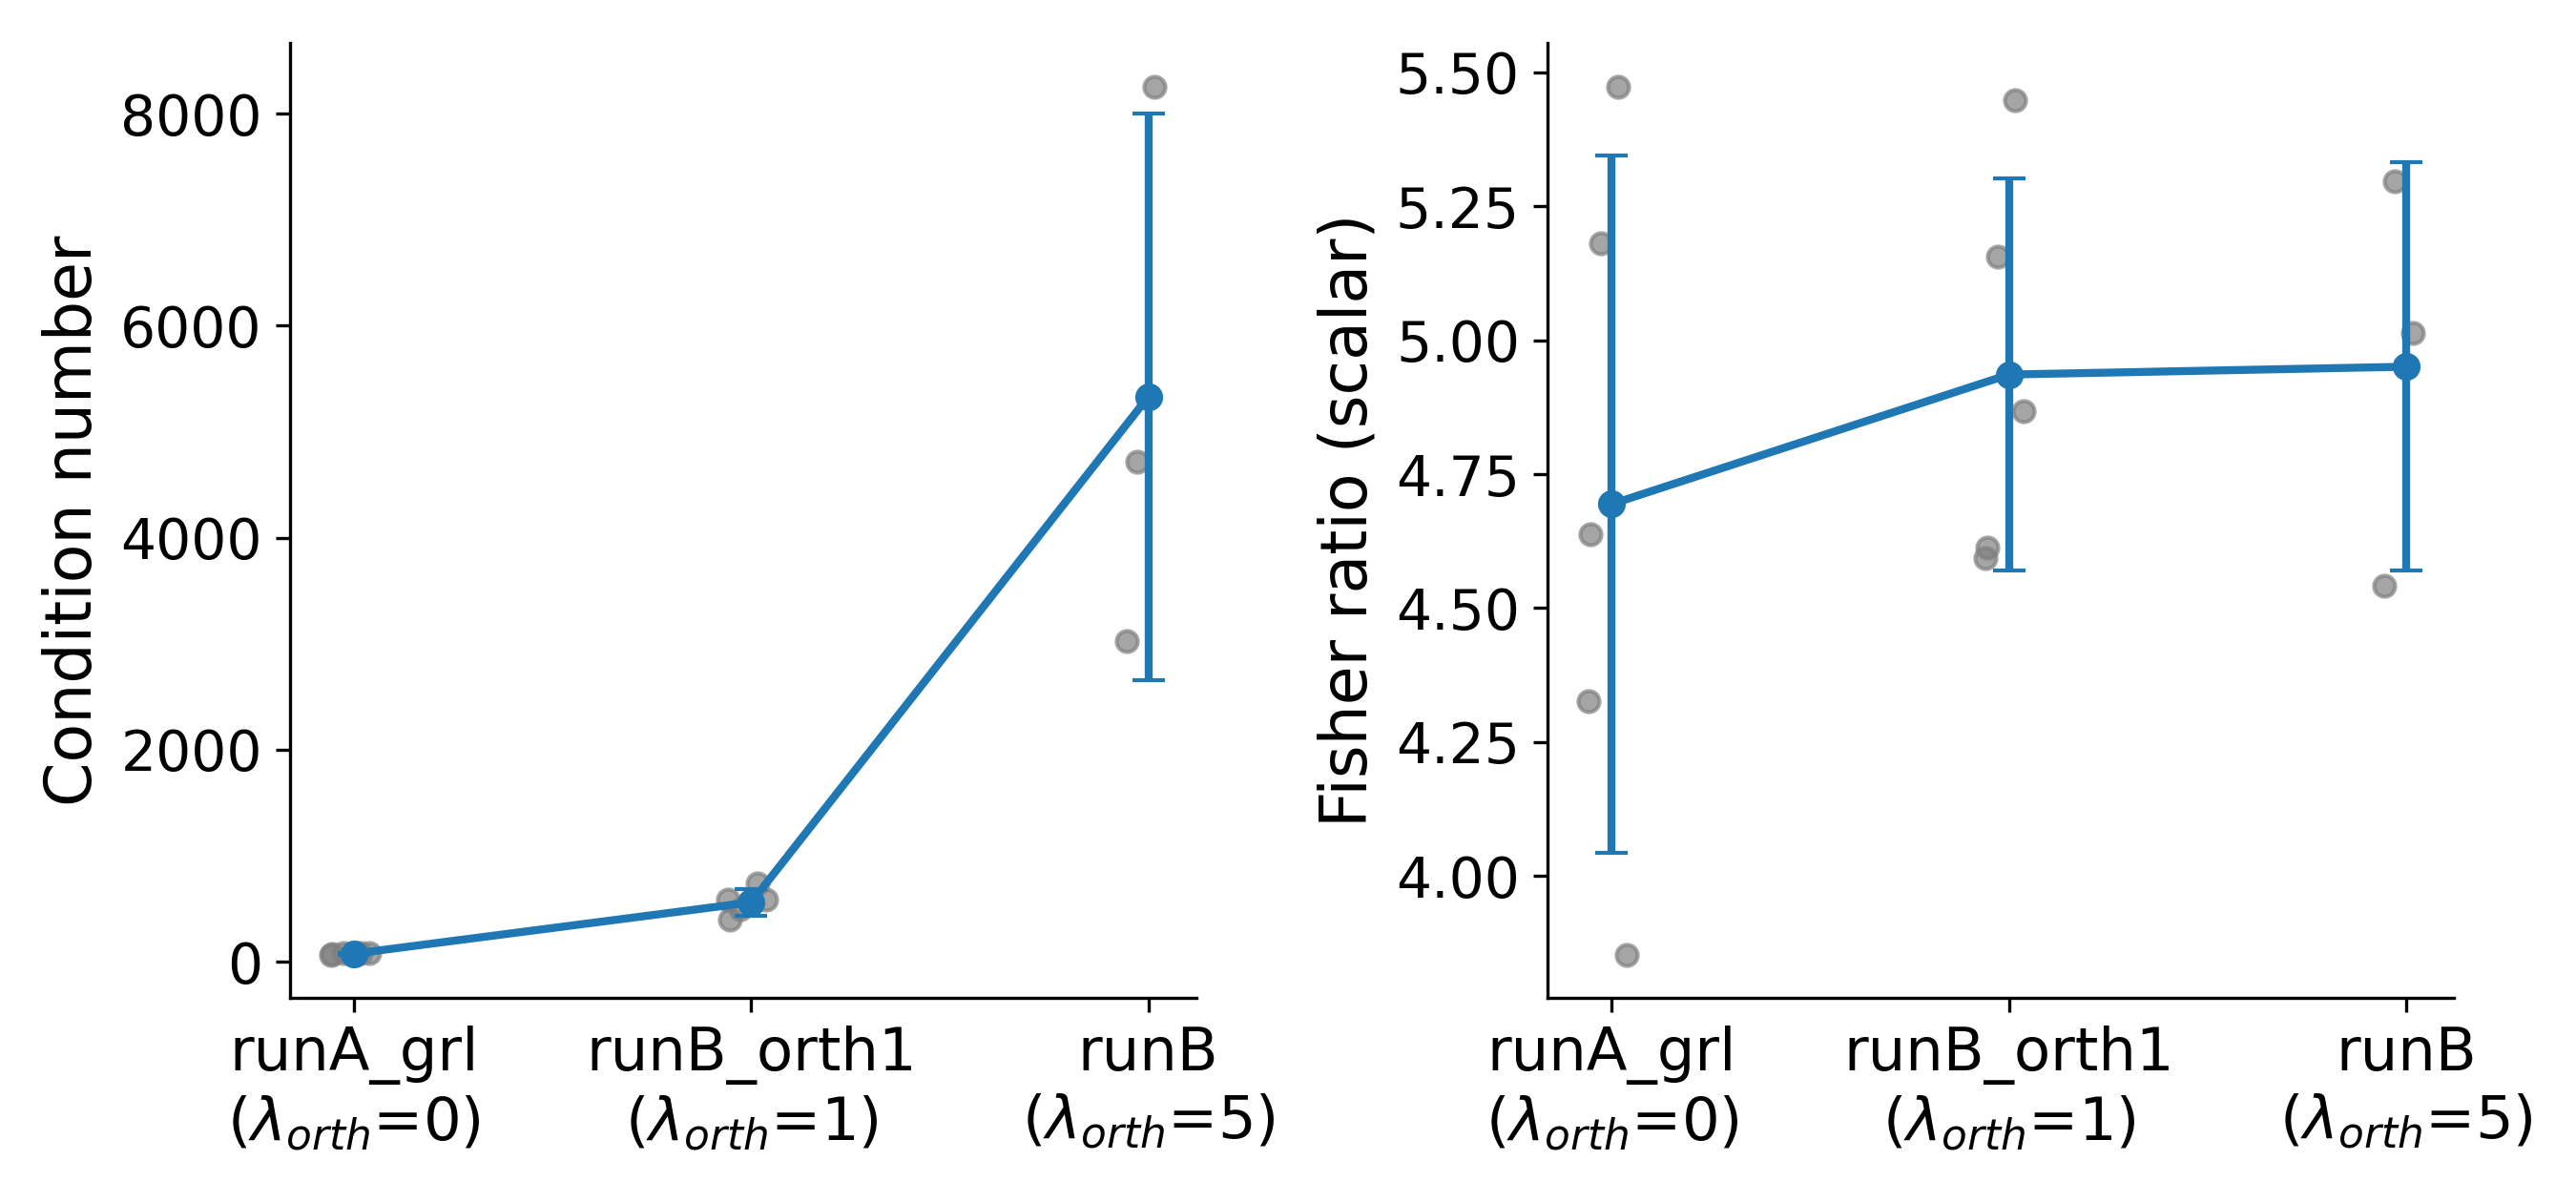
\includegraphics[width=\textwidth]{figures/figure_ladder_trend.png}
\caption{Representation geometry across the disentanglement ladder. Condition number (left) and the decoupled Fisher-ratio scalar $\mathrm{tr}(S_B)/\mathrm{tr}(S_W)$ (right) for each of 13 checkpoints (gray points; mean $\pm$ SD in blue), across three levels of orthogonality strength. Condition number increases by approximately two orders of magnitude with $\lambda_{orth}$ (Kendall's $\tau=0.84$, exact $p=2.8\times10^{-5}$; Table~\ref{tab:geometry-summary}); the Fisher-ratio scalar shows no significant trend. The remaining three geometry metrics (Fisher ratio, Hotelling--Lawley form; Mardia's kurtosis $b$ and $z$) are in Supplementary Figure~S1.}
\label{fig:ladder-trend}
\end{figure}

\subsection{Representation geometry shows no measurable association with Mahalanobis AUROC}
\label{sec:results-geometry-auroc}

Mahalanobis AUROC (ISIC-test vs.\ PAD-UFES) was $0.401\pm0.028$ (\texttt{runA\_grl}), $0.408\pm0.022$ (\texttt{runB\_orth1}), and $0.393\pm0.025$ (\texttt{runB})---below the chance value of 0.5 at every rung (Table~\ref{tab:mahalanobis-auroc}).

None of the five geometry metrics, including condition number, showed a significant association with Mahalanobis AUROC: condition number, $\tau=-0.13$, $p=0.59$; Fisher ratio (HL), $\tau=-0.28$, $p=0.20$; Fisher ratio (scalar), $\tau=-0.15$, $p=0.51$; Mardia's kurtosis ($b$), $\tau=-0.13$, $p=0.59$; Mardia's kurtosis ($z$), $\tau=-0.13$, $p=0.59$ (Figure~\ref{fig:geometry-vs-auroc}). AUROC itself showed no significant trend across the ladder (Jonckheere--Terpstra, $J=25.0$ against a null mean of 27.5, exact $p=0.65$).

An approximately two-orders-of-magnitude change in condition number (Section~\ref{sec:results-geometry}) is not accompanied by a significant change in Mahalanobis AUROC; no geometry metric tested shows a significant association with AUROC.

% table_mahalanobis_auroc.tex -- from results/table2_e2_summary.csv
% \input from sections/results.tex, Section~\ref{sec:results-geometry-auroc}.
\begin{table}[htbp]
\centering
\caption{Mahalanobis-distance AUROC (ISIC-test vs.\ PAD-UFES), by rung (mean $\pm$ SD across seeds).}
\label{tab:mahalanobis-auroc}
\begin{tabular}{lcccc}
\toprule
Rung & $\lambda_{orth}$ & $n$ seeds & AUROC & FPR@95\%TPR \\
\midrule
\texttt{runA\_grl}   & 0 & 5 & $0.401 \pm 0.028$ & $0.985 \pm 0.009$ \\
\texttt{runB\_orth1} & 1 & 5 & $0.408 \pm 0.022$ & $0.980 \pm 0.012$ \\
\texttt{runB}        & 5 & 3 & $0.393 \pm 0.025$ & $0.985 \pm 0.003$ \\
\bottomrule
\end{tabular}
\end{table}


\begin{figure}[htbp]
\centering
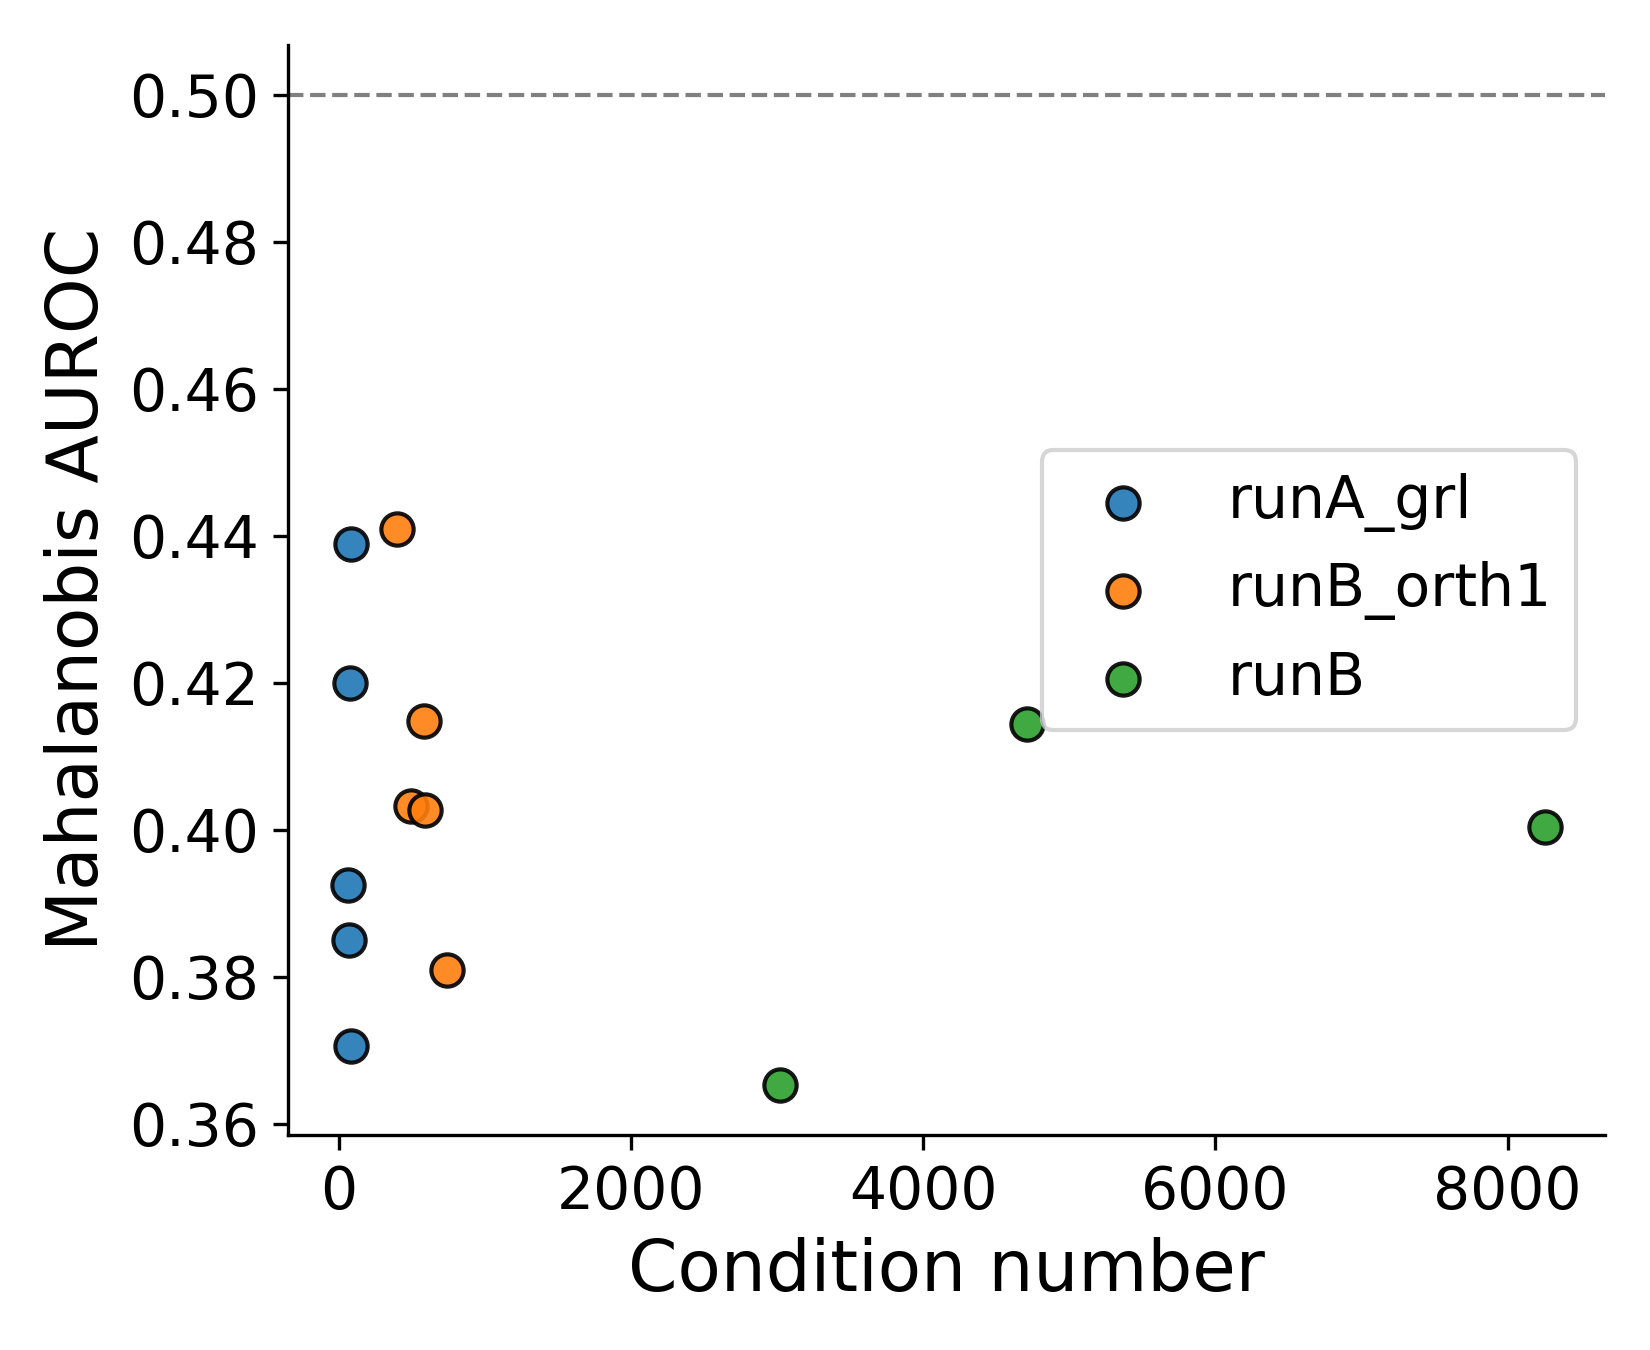
\includegraphics[width=0.6\textwidth]{figures/figure_geometry_vs_auroc.png}
\caption{Representation geometry does not predict Mahalanobis AUROC. Condition number vs.\ Mahalanobis-distance AUROC (ISIC-test vs.\ PAD-UFES), one point per checkpoint, colored by rung. No association is apparent (Kendall's $\tau=-0.13$, $p=0.59$; Table~\ref{tab:mahalanobis-auroc}); the remaining four geometry metrics show the same pattern (Supplementary Figure~S2).}
\label{fig:geometry-vs-auroc}
\end{figure}

\subsection{Distance-based scores are systematically lower for the target domain}
\label{sec:results-distance-gap}

Median Mahalanobis squared distance was lower for PAD-UFES than for ISIC-test at every one of the 13 checkpoints. Pooled across seeds within each rung: \texttt{runA\_grl}, ISIC-test median 13.50 vs.\ PAD-UFES median 8.57 ($n_{id}=25335$, $n_{ood}=11490$); \texttt{runB\_orth1}, 14.10 vs.\ 8.99 ($n_{id}=25335$, $n_{ood}=11490$); \texttt{runB}, 13.20 vs.\ 8.08 ($n_{id}=15201$, $n_{ood}=6894$). Median distance was lower for the target domain than the source domain at all 13 checkpoints.

Feature-norm distributions differed modestly between domains. Pooled median $\|z\|$: \texttt{runA\_grl}, ISIC-test 6.31 vs.\ PAD-UFES 6.21; \texttt{runB\_orth1}, 6.38 vs.\ 6.28; \texttt{runB}, 6.28 vs.\ 5.97. At the level of pooled means, the direction was not consistent across rungs (\texttt{runA\_grl} mean: 6.72 ISIC-test vs.\ 6.83 PAD-UFES). The direction of this difference was not consistent at the level of means.

Nearest-centroid classification assigned PAD-UFES samples to the majority ISIC class (Nevus) at 61.6\% (\texttt{runA\_grl}), 61.9\% (\texttt{runB\_orth1}), and 63.9\% (\texttt{runB}), compared to 53.0\%, 53.1\%, and 53.4\% respectively for ISIC-test samples classified against their own nearest centroid. This was 8.7--10.5 percentage points higher than the ISIC-test baseline rate (ratio 1.16--1.20).

\begin{figure}[htbp]
\centering
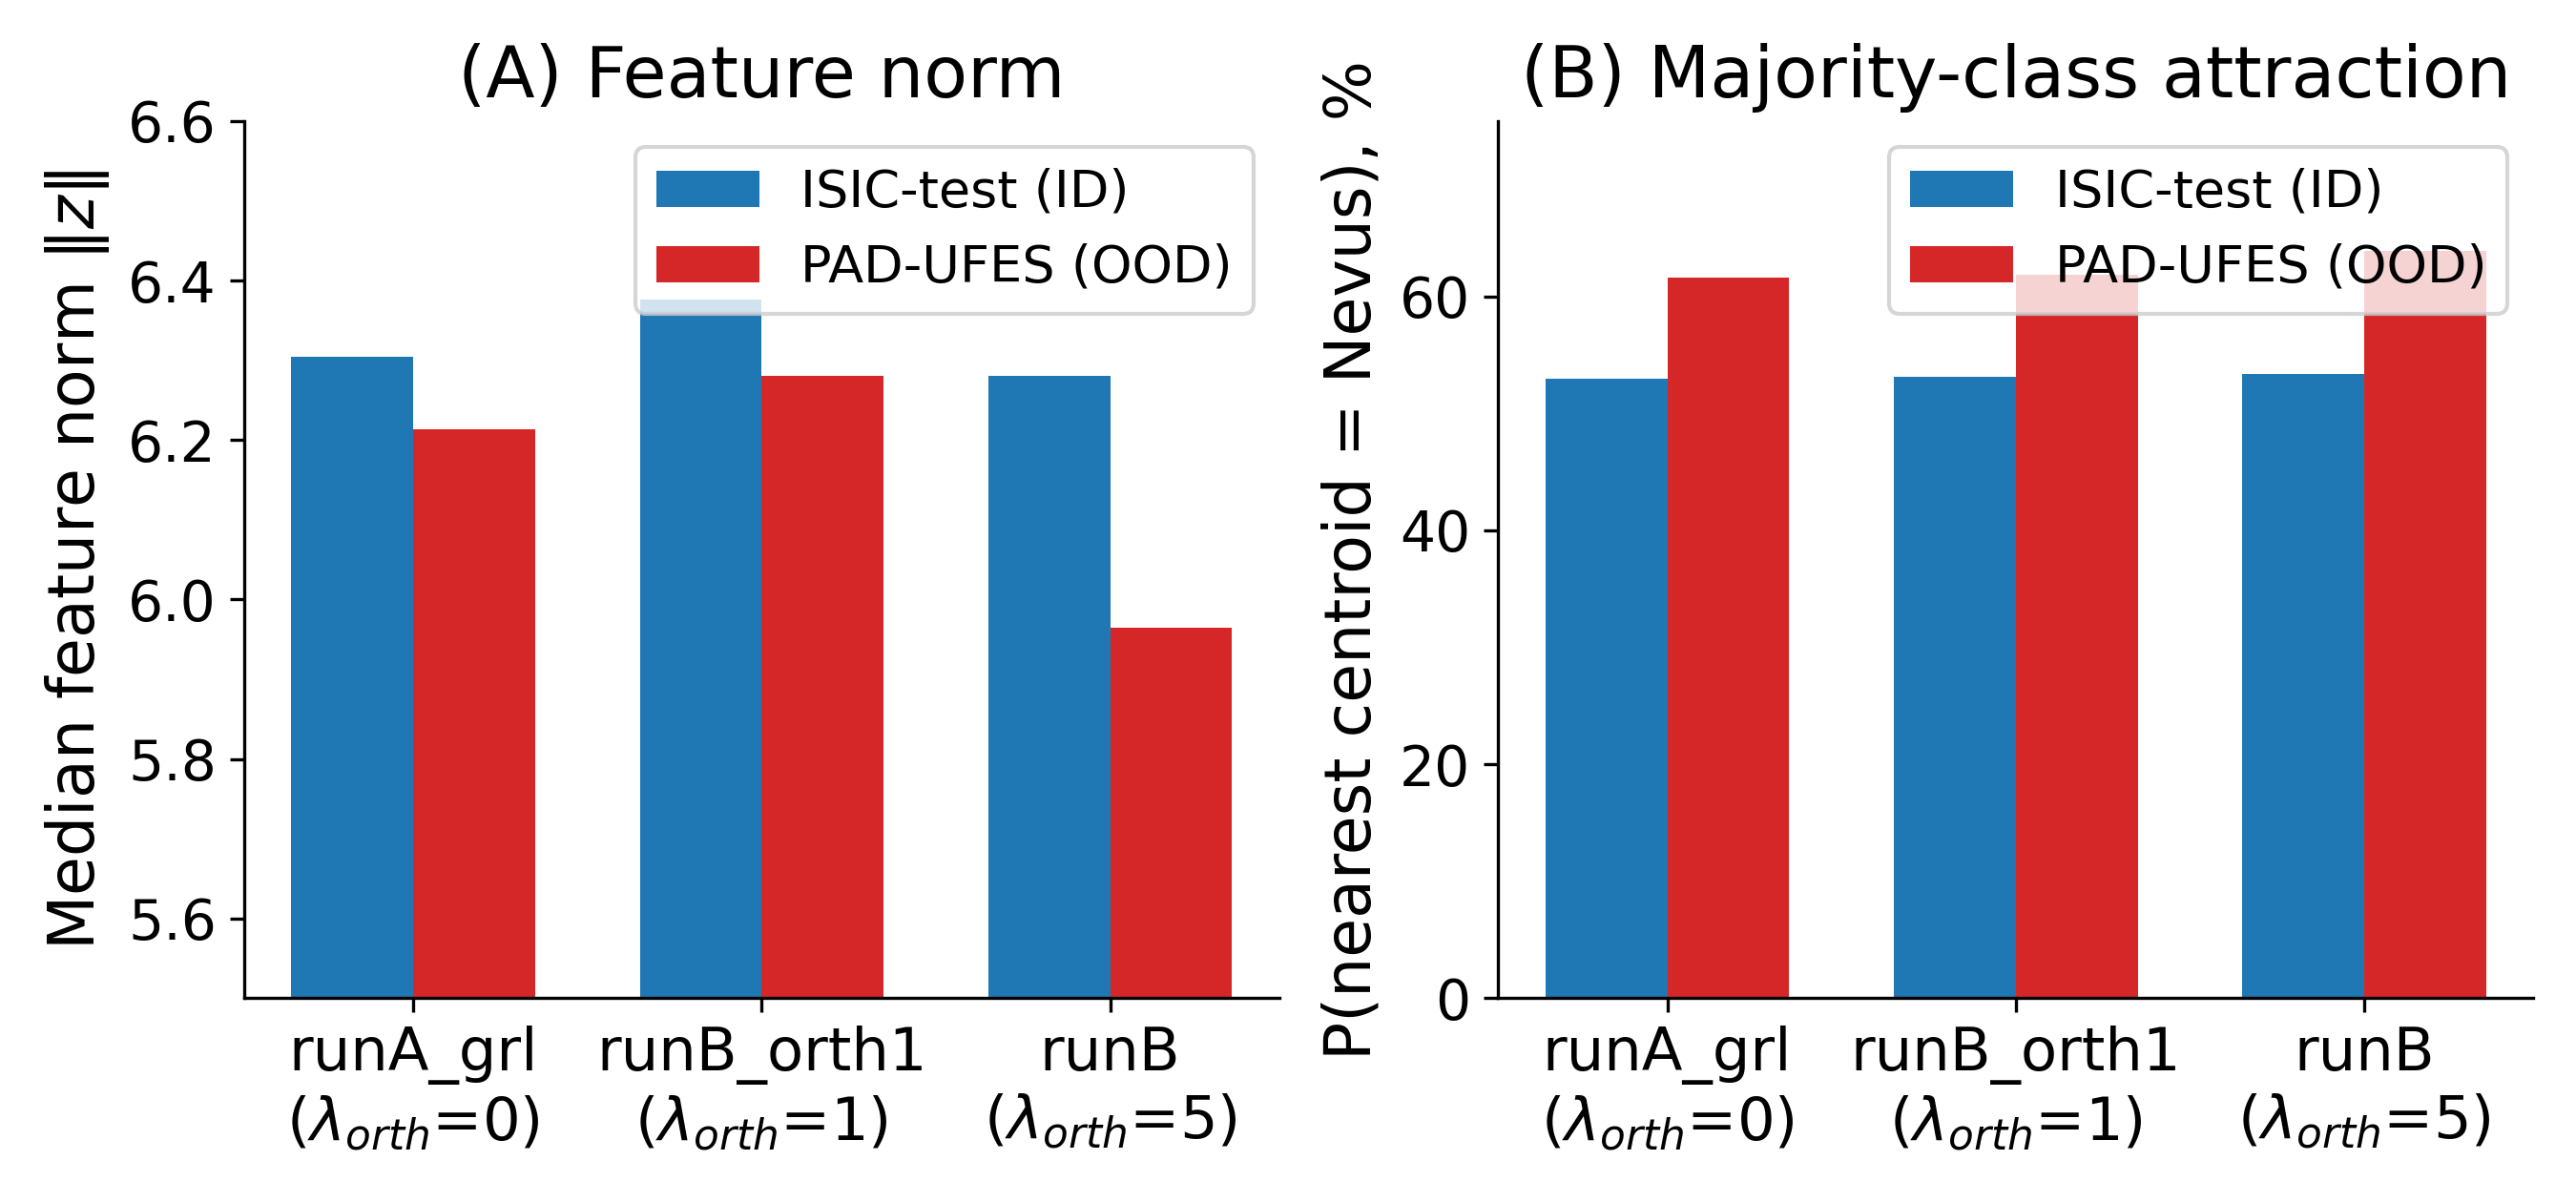
\includegraphics[width=\textwidth]{figures/figure_mechanism.png}
\caption{Neither feature-norm difference nor majority-class attraction fully accounts for the raw ID/OOD distance gap. (A) Pooled median feature norm, ISIC-test vs.\ PAD-UFES, per rung. (B) Nearest-centroid assignment of ISIC-test and PAD-UFES samples to the majority ISIC class (Nevus), per rung. The norm difference is modest and not consistent in direction at the level of means; PAD-UFES's excess attraction to the majority class (8.7--10.5 percentage points above the ISIC-test baseline) is real but does not, on its own, account for the full distance separation in Figure~\ref{fig:scorer-comparison}.}
\label{fig:mechanism}
\end{figure}

\subsection{The failure generalizes across eight scorer families}
\label{sec:results-scorer-comparison}

Pooled across all 13 checkpoints, AUROC was $0.402\pm0.024$ (Mahalanobis), $0.418\pm0.022$ (cosine-to-centroid), $0.424\pm0.023$ ($k$-NN, $k=1$), $0.414\pm0.024$ ($k$-NN, $k=10$), and $0.411\pm0.023$ ($k$-NN, $k=50$) (Table~\ref{tab:scorer-summary}, Figure~\ref{fig:scorer-comparison}). All five values fall within a 0.40--0.42 range and below the chance value of 0.5. Despite relying on substantially different scoring formulations---parametric with covariance, parametric without covariance, and non-parametric---all five distance-based scorer families produced highly similar AUROC values.

To test whether this failure is specific to distance-based scoring, we additionally evaluated three scorers that are not distance-based: Energy (a logit-based confidence score), ViM (Virtual-Logit Matching, a residual-subspace scorer that combines geometry and logits), and a per-class kernel density estimator. Pooled across the same 13 checkpoints, AUROC was $0.447\pm0.047$ (Energy), $0.387\pm0.022$ (ViM), and $0.417\pm0.025$ (density estimator)---all three within the same 0.39--0.45 range as the five distance-based scorers, and below or near the chance value of 0.5.

None of the five distance-based scorer variants showed a significant association with $\lambda_{orth}$: Mahalanobis, $\tau=-0.08$, $p=0.80$; cosine, $\tau=0.32$, $p=0.19$; $k$-NN ($k=1$), $\tau=-0.05$, $p=0.90$; $k$-NN ($k=10$), $\tau=0.02$, $p=1.00$; $k$-NN ($k=50$), $\tau=0.08$, $p=0.80$. Jonckheere--Terpstra trend testing gave the same result for all five (exact $p$ between 0.10 and 0.65). Among the three additional scorers, ViM ($\tau=0.08$, $p=0.80$) and the density estimator ($\tau=0.02$, $p=1.00$) likewise showed no significant association. Energy exhibited a modest monotonic trend with increasing disentanglement (Kendall's $\tau=0.44$, exact $p=0.065$; Jonckheere--Terpstra $p=0.032$), whereas the remaining seven scorers showed no consistent trend (full statistics in Supplementary Table~S7).

Eight structurally distinct scorers---five distance-based (parametric with and without covariance, and non-parametric $k$-NN at three values of $k$) and three that are not distance-based (a logit-based confidence score, a residual-subspace scorer, and a non-parametric density estimator)---report AUROC in essentially the same 0.39--0.45 range, all at or below chance, with one exception (Energy's Jonckheere--Terpstra trend) discussed in Section~\ref{sec:discussion}.

% table_scorer_summary.tex -- from results/table_e2_6_scorer_summary.csv
% \input from sections/results.tex, Section~\ref{sec:results-scorer-comparison}.
\begin{table}[htbp]
\centering
\caption{AUROC (ISIC-test vs.\ PAD-UFES) for eight scorers, by rung and pooled (mean $\pm$ SD across seeds).}
\label{tab:scorer-summary}
\begin{tabular}{lcccc}
\toprule
Scorer & \texttt{runA\_grl} & \texttt{runB\_orth1} & \texttt{runB} & Pooled ($n=13$) \\
\midrule
\multicolumn{5}{l}{\textit{Distance-based}} \\
Mahalanobis         & $0.401 \pm 0.028$ & $0.408 \pm 0.022$ & $0.393 \pm 0.025$ & $0.402 \pm 0.024$ \\
Cosine-to-centroid  & $0.411 \pm 0.020$ & $0.413 \pm 0.015$ & $0.439 \pm 0.027$ & $0.418 \pm 0.022$ \\
$k$-NN ($k=1$)      & $0.424 \pm 0.028$ & $0.428 \pm 0.020$ & $0.416 \pm 0.028$ & $0.424 \pm 0.023$ \\
$k$-NN ($k=10$)     & $0.413 \pm 0.029$ & $0.417 \pm 0.020$ & $0.408 \pm 0.029$ & $0.414 \pm 0.024$ \\
$k$-NN ($k=50$)     & $0.411 \pm 0.027$ & $0.414 \pm 0.020$ & $0.408 \pm 0.030$ & $0.411 \pm 0.023$ \\
\midrule
\multicolumn{5}{l}{\textit{Non-distance-based}} \\
Energy              & $0.429 \pm 0.044$ & $0.429 \pm 0.022$ & $0.506 \pm 0.035$ & $0.447 \pm 0.047$ \\
ViM                 & $0.381 \pm 0.007$ & $0.392 \pm 0.036$ & $0.386 \pm 0.014$ & $0.387 \pm 0.022$ \\
Density (KDE)       & $0.416 \pm 0.029$ & $0.420 \pm 0.022$ & $0.412 \pm 0.031$ & $0.417 \pm 0.025$ \\
\bottomrule
\end{tabular}
\end{table}


\begin{figure}[htbp]
\centering

\includegraphics[width=\textwidth]{figures/figure_e2_6_scorer_comparison.png}
\caption{Eight scorers fail alike, with one isolated exception. AUROC (ISIC-test vs.\ PAD-UFES) for five distance-based scorers (Mahalanobis distance, cosine-to-centroid similarity, pooled $k$-nearest-neighbor distance at $k=1,10,50$) and three non-distance-based scorers (Energy, ViM, per-class KDE density), computed on the identical embeddings, grouped by rung (mean $\pm$ SD across seeds). Dashed line: chance (AUROC = 0.5); dotted line separates the two scorer families. Seven of eight scorers fall within a 0.39--0.42 range with no significant trend; Energy alone rises with $\lambda_{orth}$ (Jonckheere--Terpstra exact $p=0.032$), discussed in Section~\ref{sec:discussion} as an isolated, hypothesis-generating observation (Table~\ref{tab:scorer-summary}).}
\label{fig:scorer-comparison}
\end{figure}

\subsection{Domain information remains decodable despite distance-based inaccessibility}
\label{sec:results-probe}

On the identical embeddings scored in Section~\ref{sec:results-scorer-comparison}, three supervised probes recovered domain membership (ISIC-test vs.\ PAD-UFES) at: \texttt{runA\_grl}, 0.719 (logistic regression), 0.717 (linear SVM), 0.807 (random forest); \texttt{runB\_orth1}, 0.741, 0.740, 0.815; \texttt{runB}, 0.750, 0.751, 0.800 (Table~\ref{tab:probe-vs-distance}, Figure~\ref{fig:dumbbell}). AUROC exceeded 0.70 for all three probe families at every rung.

None of the three probes showed a significant association with $\lambda_{orth}$: logistic regression, $\tau=0.26$, $p=0.30$; linear SVM, $\tau=0.26$, $p=0.30$; random forest, $\tau=-0.11$, $p=0.70$.

Three independent classifiers, applied to the same embeddings scored by the eight non-probing scorers in Section~\ref{sec:results-scorer-comparison}, recover domain membership at 0.72--0.81 AUROC at every $\lambda_{orth}$ level tested; probe AUROC shows no significant association with $\lambda_{orth}$.

% table_probe_vs_distance.tex -- from results/table_e2_7_domain_vs_distance.csv
% \input from sections/results.tex, Section~\ref{sec:results-probe} and
% Section~\ref{sec:results-baseline}. The baseline_soft row is visually
% separated (midrule + role column) so it is never read as a fourth ladder
% point -- matches the rule that it never shares an axis/table block with
% the ladder without being marked as a categorical reference.
%
% The primary-ladder pooled column now averages over all eight scorers in
% Table~\ref{tab:scorer-summary} (E2.6's five distance-based plus E2.8's
% Energy/ViM/density), not just the original five -- baseline_soft's own
% pooled value still reflects only the five E2.6 scorers, since E2.8 was
% scoped to the primary ladder only (Section~\ref{sec:results-scorer-comparison}).
\begin{table}[htbp]
\centering
\caption{Non-probing scorer AUROC (pooled across Table~\ref{tab:scorer-summary}) vs.\ domain-probe AUROC, by rung. \texttt{baseline\_soft} is a descriptive reference, not a fourth ladder point (Section~\ref{sec:ladder}).}
\label{tab:probe-vs-distance}
\resizebox{\textwidth}{!}{%
\begin{tabular}{llcccc}
\toprule
Rung & Role & Scorers (pooled) & Probe (LR) & Probe (SVM) & Probe (RF) \\
\midrule
\texttt{runA\_grl}   & primary ladder & $0.411$ & $0.719$ & $0.717$ & $0.807$ \\
\texttt{runB\_orth1} & primary ladder & $0.415$ & $0.741$ & $0.740$ & $0.815$ \\
\texttt{runB}        & primary ladder & $0.421$ & $0.750$ & $0.751$ & $0.800$ \\
\midrule
\texttt{baseline\_soft} & categorical reference ($n=1$) & $0.828$ & $0.998$ & $0.997$ & $0.977$ \\
\bottomrule
\end{tabular}%
}
\end{table}


\begin{figure}[htbp]
\centering
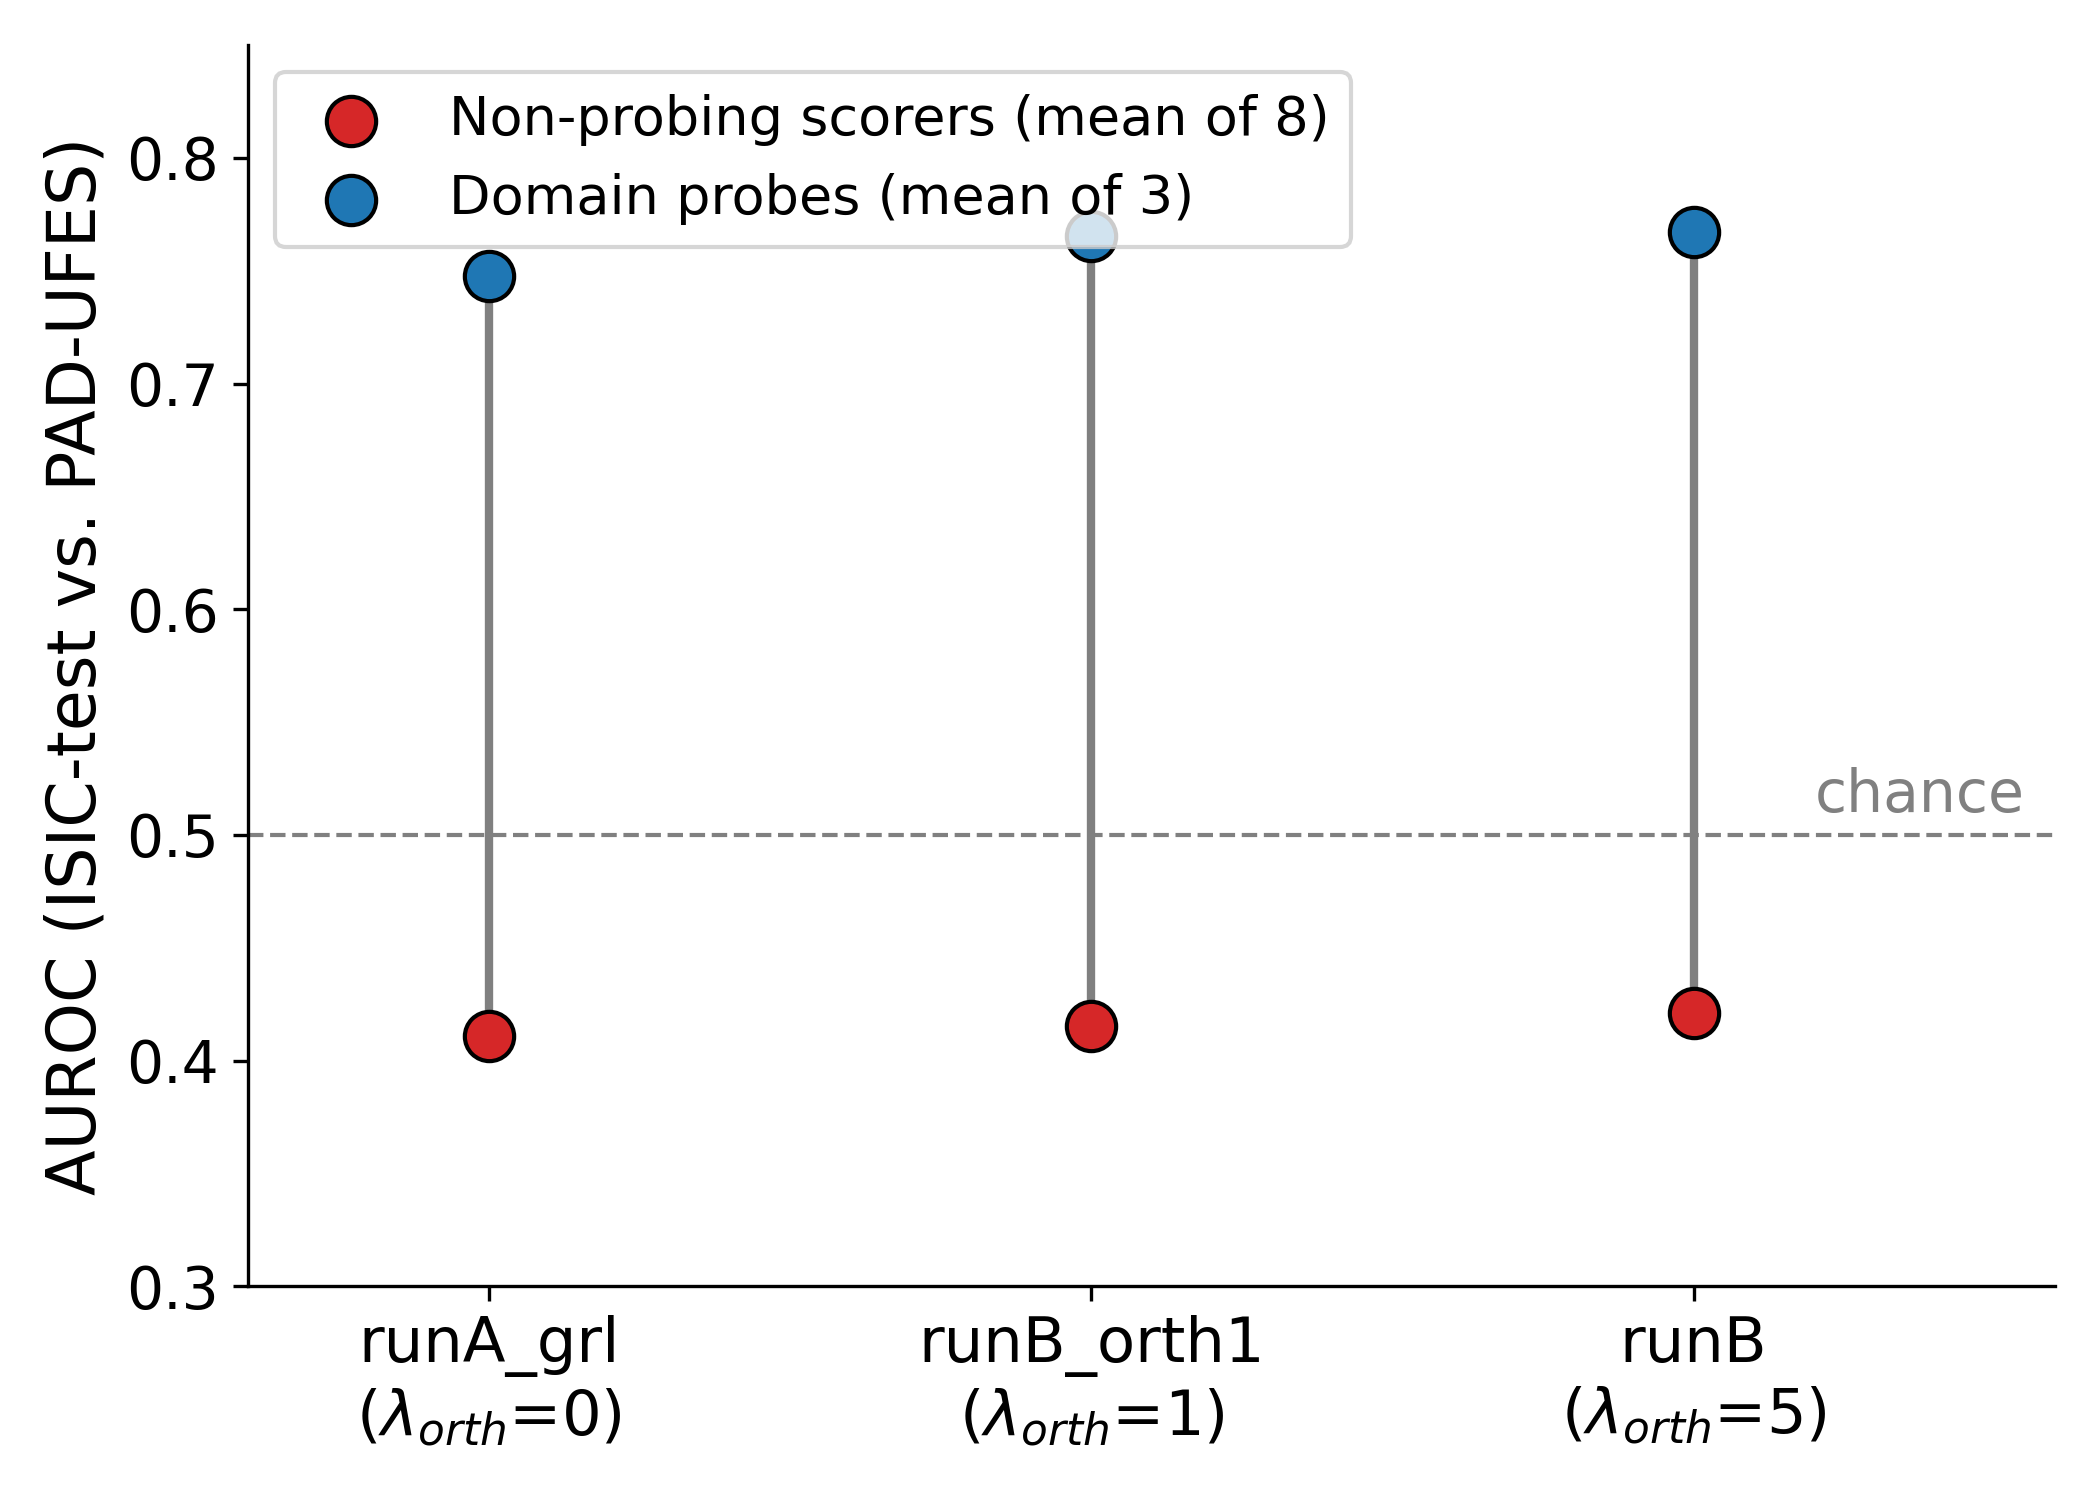
\includegraphics[width=0.8\textwidth]{figures/figure_dumbbell.png}
\caption{Domain information is decodable but not accessible to non-probing scorers. For each rung, mean AUROC across the eight scorers in Figure~\ref{fig:scorer-comparison} (five distance-based, three non-distance-based) is connected to mean AUROC across three independent domain probes---logistic regression, linear SVM, random forest (Section~\ref{sec:probe})---computed on the identical embeddings. Non-probing scorers cluster at or below chance ($\approx 0.41$); probes recover domain membership at 0.72--0.81 AUROC at every $\lambda_{orth}$ level. \texttt{baseline\_soft} (Section~\ref{sec:results-baseline}) is not plotted on this axis, as it is a descriptive reference confounded by architecture and dimensionality (Section~\ref{sec:ladder}), not a controlled comparison point.}
\label{fig:dumbbell}
\end{figure}

\subsection{Descriptive reference: a non-disentangled baseline}
\label{sec:results-baseline}

For a single ResNet-50 checkpoint (\texttt{baseline\_soft}; one seed, architecture and representation dimensionality differing from the ladder, Section~\ref{sec:ladder}), pooled AUROC across the five distance-based scorers was 0.828 (the three non-distance-based scorers were not evaluated on this architecture, Section~\ref{sec:results-scorer-comparison}), and probe AUROC was 0.998 (logistic regression), 0.997 (linear SVM), and 0.977 (random forest) (Table~\ref{tab:probe-vs-distance}).
